While the knowledge representation presented in this paper provides the \lq\lq{}slots\rq\rq{} necessary for representing dynamic information, the
static file structure makes the utilization of these slots awkward. It is desirable to be able to represent the dynamic information in a dynamic database.
For this reason, the authors have developed a technique for automatically generating tables for storing,  and access functions
for obtaining, the data from the ontology in a MySQL database.

Reading data from and to the MySQL database instead of the ontology file offers the community easy access to a live data structure. Furthermore, it is more practical to modify the information stored in a database than if it was stored in an ontology, which in some cases, requires the deletion and re-creation of the whole file. A literature review reveals many efforts and methodologies that have been designed to produce SQL databases from ontologies. Our effort builds upon the work of Astrova et al.\cite{Astrova2007}. 

In addition to generating and filling the database tables, the authors have created tools that automatically generate a set of C++ classes for reading and writing
information to the kitting MySQL database. The choice of C++ was a team preference and we believe that other object-oriented languages could have been used in this project.

The Generator tool is a graphical user interface developed in Java, allowing the user to store data from OWL files into a MySQL database. This tool also permits the user to query the database using the C++ function calls. The tool Generator is composed of the following functionalities:
\begin{enumerate}
 \item Convert OWL documents into SQL syntaxes (OWL to SQL).
 \item Translate SQL syntaxes to OWL language in order to modify an OWL document (SQL to OWL).
 \item Convert the OWL language into C++ classes (OWL to C++).
\end{enumerate}

To date, only steps 1. and 3. have been implemented and will be covered in this document.
In order to generate the SQL database and C++ classes, the OWL object model must be mapped to the C++ object model and the relational SQL model. 
To quote the OWL 2 Web Ontolongy website~\cite{OWLspec}, ``Entities are the fundamental building blocks of OWL 2 ontologies, 
and they define the vocabulary --the named terms-- of an ontology. In logic, the set of entities is usually said to constitute the 
signature of an ontology''. Therefore, the notions of single-valued and multi-valued properties as well as the inheritance must be 
mapped from the ontolongy to the SQL database and C++ classes. The mapping from OWL proceeds as follows:
\begin{itemize}
\item Data properties: In an ontology, data properties link an individual to a data value. Single-valued data properties are mapped into a SQL table entry or C++ class
variable with the corresponding type of the original property. For example, in the ontology a robot has a single-valued data 
property \texttt{hasRobot\_Description}, represented in the
SQL database as a \texttt{varchar} and in the corresponding C++ class as \texttt{std:string}. 
Multi-valued data properties are mapped from the ontology into the SQL database as a table and into the C++ class as a \texttt{std:vector} with the corresponding
type of the original property. For example,
in the ontology a stock keeping unit has a multi-valued
data property \texttt{hasSku\_EndEffectorRefs}. This maps to a SQL table containing \texttt{varchar} entries and the C++
\texttt{std::vector\textless std::string\textgreater} in the corresponding C++ class.

\item Object property: In an ontology, object properties link one individual to another individual. 
The single-valued object properties are mapped to a SQL table entry or C++ class
variable. Their type is a pointer to the range of the object properties. For example, in the ontology a solid object has the object property \texttt{hasRobot\_Description} 
linking it to a physical location. In the SQL database, ??? In the C++ classes, this is represented by a reference to a physical location: \texttt{PhysicalLocation* hasSolidObject\_PrimaryLocation}.
Multi-valued object properties are mapped from the ontology into the SQL database as a table and into the C++ class as a \texttt{std:vector} of pointers referencing objects of the range of the property.  For example, a solid object also has a list of secondary locations corresponding to a multi-valued object property in the ontology: {\scriptsize\texttt{std::vector\\ \textless PhysicalLocation*\textgreater hasSolidObject\_SecondaryLocation}}.
\end{itemize}

\subsection{MySQL Database Generation}\label{ss:ontology2db}
\begin{figure}[h!t!]
\centering
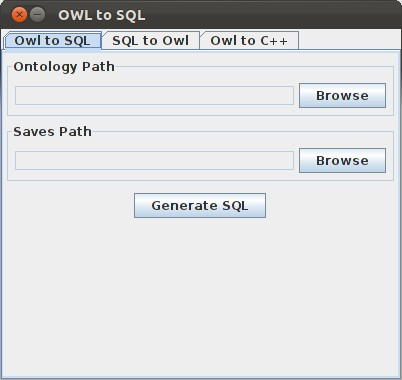
\includegraphics[width=8.5cm]{images/OWLtoSQL001.jpeg}
\caption{Owl to SQL tab.}
\label{fig:owl2sql}
\end{figure}

This section provides basic information on the Generator Java tool. Specific information on the tools usage is included with the tool in its manual.
Converting an OWL ontology to SQL script files is easily performed using the \texttt{Owl to SQL} tab  (see Figure~\ref{fig:owl2sql}). The required fields are:

\begin{itemize}
 \item Ontology Path: The OWL file to be converted. Note that all \texttt{Import} statements in this file must use absolute paths.
 \item Saves Path: The directory where you want to save the SQL files.
\end{itemize}

Clicking on the ``Generate SQL'' will generate the SQL script files. Two files will be created by the tool:
\begin{itemize}
\item The file used to create tables in the database: \texttt{<inputfile>.owlCreateTable.sql} 
\item The file used to populate the database tables: \texttt{<inputfile>.owlInsertInto.sql}. 
\end{itemize}
These files may then be used with the SQL command line interface to create and populate the database.

\subsection{C++ Class Generation and Usage}
As previously mentioned, the C++ classes are automatically generated by the Generator tool. In addition to the class structure, 
Data Access Objects (DAO) that are needed to interact with the MySQL database are generated. 
To map the MySQL database and indirectly the ontology to C++ classes, both the C++ classes and
the DAO must be generated.

The C++ class files (.cpp) and header files (.h) are generated in a two step process.
The first step does not depend on the content of the ontology, it only initializes the specific objects related to the MySQL connector driver
(see Figure~\ref{fig:headerclass}).

The second step generates all the C++ headers and class files relative to our ontology. 
All of the \texttt{include} statements  are made directly in the C++ class files, and only forward declarations are performed in the headers. 
This resolves problems associated with circular includes or multiple includes. All of the classes include the following methods:
\begin{itemize}
\item \texttt{This should include all of the methods that a user may need to call and a description of them.}
\item \texttt{getter} - some description of what this does
\item \texttt{setter} - some description of what this does
\item \texttt{explode} - method that splits a string into a vector around matches of a given regular expression, 
\item \texttt{copy} -  method that takes a C++ map as input and copy the values from the map into the instance. 
\item \texttt{get} - reads data from the MySQL database,
\item \texttt{set} - writes data to the MySQL database,
\item \texttt{init} - Does this really exist? methods that initialize and use the DAO.
\end{itemize}

\begin{figure}[t!h!]
\begin{minipage}{.5\paperwidth}
\begin{mylisting}
\begin{Verbatim}[commandchars=\\\{\},fontsize=\scriptsize, numbersep=2pt]
\textbf{#ifndef} PARTSBIN_H_
\textbf{#define} PARTSBIN_H_
\textbf{#include} <cstdlib>
\textbf{#include} <iostream>
\textbf{#include} <map>
\textbf{#include} <string>
\textbf{#include} <vector>
\textbf{#include} <sstream>

\textbf{#include} "BoxyObject.h"
\textbf{class} DAO;
\textbf{class} PartsBin: \textbf{public} BoxyObject \{
    \textbf{private}:
        std::string hasBin_PartQuantity;
        std::string hasBin_PartSkuRef;
        \textbf{int} PartsBinID;
        DAO* dao;
    \textbf{public}:
        PartsBin(std::string name);
        ~PartsBin();
        \textbf{void} get(\textbf{int} id);
        \textbf{void} get(std::string name);
        \textbf{void} set(\textbf{int} id, PartsBin* obj);
        \textbf{void} set(std::string name);
        std::string gethasBin_PartQuantity();
        \textbf{void} sethasBin_PartQuantity(
            std::string _hasBin_PartQuantity);
        std::string gethasBin_PartSkuRef();
        \textbf{void} sethasBin_PartSkuRef(
            std::string _hasBin_PartSkuRef);
        \textbf{int} getPartsBinID();
        DAO* getdao();
        \textbf{void} setdao(DAO* _dao);
        \textbf{void} copy(std::map<std::string,
            std::string> object);
        std::vector<std::string> Explode(
            \textbf{const} std::string & str, \textbf{char} separator);
\};
\textbf{#endif} /* PARTSBIN_H_ */
\end{Verbatim}
\end{mylisting}
\end{minipage}
\caption{Header of a generated class.}
\label{fig:headerclass}
\end{figure}



%\lstset{frame=single, language=C++, caption=Header of a generated class, label=Header of a generated class,
%captionpos=b}
%\begin{lstlisting}
%#ifndef PARTSBIN_H_
%#define PARTSBIN_H_
%#include <cstdlib>
%#include <iostream>
%#include <map>
%#include <string>
%#include <vector>
%#include <sstream>
%
%#include "BoxyObject.h"
%class DAO;
%class PartsBin: public BoxyObject {
%private:
%	std::string hasBin_PartQuantity;
%	std::string hasBin_PartSkuRef;
%	int PartsBinID;
%	DAO* dao;
%public:
%	PartsBin(std::string name);
%	~PartsBin();
%	void get(int id);
%	void get(std::string name);
%	void set(int id, PartsBin* obj);
%	void set(std::string name);
%	std::string gethasBin_PartQuantity();
%	void sethasBin_PartQuantity(
%		std::string _hasBin_PartQuantity);
%	std::string gethasBin_PartSkuRef();
%	void sethasBin_PartSkuRef(
%		std::string _hasBin_PartSkuRef);
%	int getPartsBinID();
%	DAO* getdao();
%	void setdao(DAO* _dao);
%	void copy(std::map<std::string, std::string> object);
%	std::vector<std::string> Explode(
%		  const std::string & str, char separator);
%};
%#endif /* PARTSBIN_H_ */
%\end{lstlisting}



The actual data access is provided through the use of a data access object (DAO).
DAOs provide an abstract interface to some type of database or other persistence
mechanism. DAOs map application calls to the database or persistence mechanism, 
thus providing some specific data operations without exposing
details of the database. The use of the DAO separates the data accesses that the application needs from how these needs can be satisfied with a specific
Database Management System (DBMS), database schema, etc.

A similar mechanism has been used in this project for the interaction between the C++ classes used by the executor module and 
The different methods of the DAO are the same for any ontology. 
The concern here is not about the data, but only about the way to retrieve or store it. Only the four vectors filled by the\texttt{fillGetSqlQueries} method differ from one 
auto-generated C++ file to another file.

When the DAO is generated, four vectors are built as follows (\ref{fig:headerdao}:

\begin{itemize}
\item line \textcolor{BrickRed}{17} : A structure with the SQL query to select the content of the tables relative to an entity, the table relative to the entity itself and the ones relative to its super classes.
\item line \textcolor{BrickRed}{18} : A structure with the SQL query to select the multi-valued attributes (multi-valued data) for a given entity.
\item line \textcolor{BrickRed}{19} : A structure with the names of the tables linked to this entity in the ontology.
\item line \textcolor{BrickRed}{20} : A structure with the names of the association tables linked to an object.
\end{itemize}

With these four structures,one is able to read (\texttt{get} method) and write (\texttt{set} method) data from and to the MySQL database. The \texttt{get} method fills 
a C++ map and gets the object itself while the \texttt{copy} method handles the data. The \texttt{set} method,is called with a C++ map containing the values of the 
different attributes as input and the \texttt{set} method writes these values into the MySQL database. \\textit{Why two set methods?}


\begin{figure}[t!h!]
\begin{minipage}{.5\paperwidth}
\begin{mylisting}
\begin{Verbatim}[commandchars=\\\{\},fontsize=\scriptsize, numbers=left, numbersep=2pt]
\textbf{#ifndef} DAO_H_
\textbf{#define} DAO_H_
\textbf{#include} <cstdlib>
\textbf{#include} <iostream>
\textbf{#include} <map>
\textbf{#include} <vector>
\textbf{#include} <sstream>

\textbf{#include} "Connection.h"
\textbf{class} DAO \{
    \textbf{private}:
      std::vector<std::string> className;
      Connection* connection;
      std::vector<std::string> nameDone;
      std::map<std::string, std::string> map;
      std::string path; std::string pathmulti;
      \textbf{static} std::map<std::string, std::string>
        getSqlQueriesDataSingle;
      \textbf{static} std::map<std::string, std::vector<std::string>>
			getSqlQueriesDataMulti;
      \textbf{static} std::map<std::string, std::vector<std::string>>
			getSqlQueriesObjectSingle;
      \textbf{static} std::map<std::string, std::vector<std::string>>
			getSqlQueriesObjectMulti;
      \textbf{static} std::map<std::string, std::vector<std::string>>
				  setSqlQueries;
      \textbf{static} std::map<std::string, std::vector<std::string>>
				updateSqlQueries;
      \textbf{void} fillGetSqlQueries();
    \textbf{public}:
      DAO(std::string name); ~DAO();
      std::vector<std::string> getclassName();
      \textbf{void} setclassName(std::vector<std::string> _className);
      Connection* getconnection();
      \textbf{void} setconnection(Connection* _connection);
      std::map<std::string,std::string> get(std::string name);
      \textbf{void} set(std::map<std::string, std::string> data);
      std::vector<std::string> Explode(\textbf{const} std::string & str,
      \textbf{char separator});
\};
\textbf{#endif} /* DAO_H_ */
\end{Verbatim}
\end{mylisting}
\end{minipage}
\caption{Header of the DAO class.}
\label{fig:headerdao}
\end{figure}


%\lstset{frame=single, language=C++, caption=Header of our DAO class, label=Header of our DAO class,
%captionpos=b}
%\begin{lstlisting}
%#ifndef DAO_H_
%#define DAO_H_
%#include <cstdlib>
%#include <iostream>
%#include <map>
%#include <vector>
%#include <sstream>
%#include "Connection.h"
%class DAO {
%private:
%	std::vector<std::string> className;
%	Connection* connection;
%	std::vector<std::string> nameDone;
%	std::map<std::string, std::string> map;
%	std::string path; std::string pathmulti;
%	static std::map<std::string, std::string>
%				  getSqlQueriesDataSingle;
%	static std::map<std::string, std::vector<std::string> >
%			getSqlQueriesDataMulti;
%	static std::map<std::string, std::vector<std::string> >
%			getSqlQueriesObjectSingle;
%	static std::map<std::string, std::vector<std::string> >
%			getSqlQueriesObjectMulti;
%	static std::map<std::string, std::vector<std::string> >
%				  setSqlQueries;
%	static std::map<std::string, std::vector<std::string> >
%				updateSqlQueries;
%	void fillGetSqlQueries();
%public:
%	DAO(std::string name); ~DAO();
%	std::vector<std::string> getclassName();
%	void setclassName(std::vector<std::string> _className);
%	Connection* getconnection();
%	void setconnection(Connection* _connection);
%	std::map<std::string,std::string> get(std::string name);
%	void set(std::map<std::string, std::string> data);
%	std::vector<std::string> Explode(const
%			std::string & str, char separator);
%};
%#endif /* DAO_H_ */
%\end{lstlisting}


\subsection{Using the C++ Classes to Access Data from the MySQL Database}

\begin{figure}[t!h!]
\begin{minipage}{.5\paperwidth}
\begin{mylisting}
\begin{Verbatim}[commandchars=\\\{\},fontsize=\scriptsize, numbers=left, numbersep=2pt]
#include "Point.h"
#include "PoseLocation.h"
#include "Vector.h"
#include "KitTray.h"

void CanonicalRobotCommand::
 getKitTrayLocation(string kit_tray_name)\{

  KitTray* kit_tray = \textbf{new} KitTray(kit_tray_name);
  kit_tray->get(kit_tray_name);

  PoseLocation* kit_tray_pose = \textbf{new} PoseLocation(
  kit_tray->gethasSolidObject_PrimaryLocation()->getname());
  kit_tray_pose->get(kit_tray_pose->getname());

  //--Retrieve hasPoseLocation_Point
  Point * kit_tray_point =
  kit_tray_pose->gethasPoseLocation_Point();

  //--Retrieve hasPoseLocation_XAxis
  Vector * kit_tray_x_axis  =
  kit_tray_pose->gethasPoseLocation_XAxis();

  //--Retrieve hasPoseLocation_ZAxis
  Vector * kit_tray_z_axis  =
  kit_tray_pose->gethasPoseLocation_ZAxis();
\}
\end{Verbatim}
\end{mylisting}
\end{minipage}
\caption{Example using the generated C++ classes.}
\label{fig:exampleofuse}
\end{figure}


%\lstset{frame=single, language=C++, caption=How to use the C++ classes, label=How to use the C++ classes,
%captionpos=b}
%\begin{lstlisting}
%KitTrayLocStruct CanonicalRobotCommand::getKitTrayLocation(string kit_tray_name){
%
%	KitTrayLocStruct kit_tray_loc_struct;
%
%	KitTray* kit_tray = new KitTray(kit_tray_name);
%	kit_tray->get(kit_tray_name);
%
%	PoseLocation* kit_tray_pose = new PoseLocation(kit_tray->gethasSolidObject_PrimaryLocation()->getname());
%	kit_tray_pose->get(kit_tray_pose->getname());
%
%	//--Retrieve hasPoseLocation_Point
%	Point * kit_tray_point = kit_tray_pose->gethasPoseLocation_Point();
%	//--Retrieve hasPoseLocation_XAxis
%	Vector * kit_tray_x_axis  = kit_tray_pose->gethasPoseLocation_XAxis();
%	//--Retrieve hasPoseLocation_ZAxis
%	Vector * kit_tray_z_axis  = kit_tray_pose->gethasPoseLocation_ZAxis();
%
%	kit_tray_loc_struct.point=kit_tray_point;
%	kit_tray_loc_struct.x_axis=kit_tray_x_axis;
%	kit_tray_loc_struct.z_axis=kit_tray_z_axis;
%
%	return kit_tray_loc_struct;
%}
%\end{lstlisting}

Figure~\ref{fig:exampleofuse} depicts an example using the generated classes to retrieve the location of the kit tray \texttt{kit\_tray\_name} from the MySQL database. The different sections of the example are described below:

\begin{itemize}
\item lines \textcolor{BrickRed}{1--4}: Include the different headers necessary to query MySQL tables. Here, the tables Point, PoseLocation, Vector, and KitTray are required.
\item line \textcolor{BrickRed}{9}: Initialize an object from the class \texttt{KitTray} by passing its name.
\item line \textcolor{BrickRed}{10}: Allow access to any data from the table KitTray.
\item lines \textcolor{BrickRed}{12--13}: Initialize an object of type \texttt{PoseLocation} and allow access to any data from the table PoseLocation.
\item lines \textcolor{BrickRed}{17--18}: Retrieve X, Y, and Z coordinates from the table Point for the kit tray \texttt{kit\_tray\_name}.
\item lines \textcolor{BrickRed}{21--22}: Retrieve the X axis vector ($X_i$, $X_j$, $X_k$) from the table Vector for the kit tray \texttt{kit\_tray\_name}.
\item lines \textcolor{BrickRed}{17--18}: Retrieve the y axis vector ($Y_i$, $Y_j$, $Y_k$) from the table Vector for the kit tray \texttt{kit\_tray\_name}.
\end{itemize}


